\documentclass[english]{exam}

\setlength {\marginparwidth }{2cm} 
\usepackage{todonotes}

\usepackage[perpage,para,symbol]{footmisc}

\hyphenpenalty=15000 
\tolerance=1000

\usepackage{tikz}
\usetikzlibrary{arrows,decorations.pathmorphing,backgrounds,fit,positioning,calc,shapes}
\usepackage{pgfmath}
\usepackage{rotating}
\usepackage{array}	
\usepackage{graphicx}
\usepackage{float}	
\usepackage{mdwlist}
\usepackage{setspace}
\usepackage{listings}
\usepackage{bytefield}
\usepackage{tabularx}
\usepackage{multirow}	       
\usepackage{caption}
\usepackage{xcolor}
\usepackage{amssymb}
\captionsetup[table]{skip=10pt}

\usepackage{url}               
\usepackage{hyperref}
\usepackage[all]{hypcap}	
\usepackage{titlesec}
\setcounter{secnumdepth}{4}
\titleformat{\paragraph}
{\normalfont\normalsize\bfseries}{\theparagraph}{1em}{}
\titlespacing*{\paragraph}
{0pt}{3.25ex plus 1ex minus .2ex}{1.5ex plus .2ex}

\definecolor{mGreen}{rgb}{0,0.6,0}
\definecolor{darkblue}{rgb}{0.1,0.1,0.5}
\definecolor{mGray}{rgb}{0.5,0.5,0.5}
\definecolor{mPurple}{rgb}{0.58,0,0.82}
\definecolor{backgroundColour}{rgb}{0.95,0.95,0.92}

\hypersetup{colorlinks,breaklinks,
            linkcolor=darkblue,urlcolor=darkblue,
            anchorcolor=darkblue,citecolor=darkblue}


\lstdefinestyle{CStyle}{
    backgroundcolor=\color{backgroundColour},   
    commentstyle=\color{mGreen},
    keywordstyle=\color{magenta},
    numberstyle=\tiny\color{mGray},
    stringstyle=\color{mPurple},
    basicstyle=\footnotesize,
    breakatwhitespace=false,         
    breaklines=true,                 
    captionpos=b,                    
    keepspaces=true,                 
    numbers=left,                    
    numbersep=5pt,                  
    showspaces=false,                
    showstringspaces=false,
    showtabs=false,                  
    tabsize=2,
    language=C
}

\PassOptionsToPackage{USenglish,english}{babel} 
\usepackage{csquotes}
\usepackage{tabto}
\usepackage[USenglish,english]{babel}
\usepackage[acronym, section=section, nonumberlist, nomain, nopostdot]{glossaries}
\makeglossaries
 
\makeglossaries
\newcommand{\colorbitbox}[3]{%
	\rlap{\bitbox{#2}{\color{#1}\rule{\width}{\height}}}%
	\bitbox{#2}{#3}}

\begin{document}

\title{Assignment II:\\ CUDA Basics}
\author{Amirhossein Namazi, Calin Capitanu}

\maketitle


\chapter{Exercise 1}
\section*{Hello World!}

The program is compiled using the compiler for CUDA programs, \textbf{nvcc}. Since the GPU that the code is ran on has the Ampere architecture (30 series Nvidia), the \textbf{-arch=sm\_80} flag is given. Finally, the source code and an output binary name are given, all resulting in this command: \\
\begin{lstlisting}
nvcc -arch=sm_80 exercise_1.cu -o exercise_1
\end{lstlisting}

\noindent

CUDA programs take advantage of the parallel processing of the GPU using CUDA Threads. These threads are independent execution threads that execute one specific action (one function, or ``kernel'' in the CUDA Jargon). These CUDA threads are grouped into CUDA thread blocks. Each thread block has the same number of threads, defined at the beginning of launching a kernel. When talking about memory management, blocks of CUDA threads can share one type of memory, while single threads also have their own memory (registers). Obviously, each thread in the thread block executes the same kernel (or function).\\\\\\

\clearpage
\chapter{Exercise 2}
\section*{Performing SAXPY on the GPU}

The problem of the number of blocks when \textbf{ARRAY\_SIZE} is not a multiple of the number of threads per block is easily fixable with the following formula for the number of blocks:\\\\
$BLOCKS = (ARRAY\_SIZE + TPB - 1) / TPB$
\\\\
This makes sure that all of the computations will have one thread to execute on, even if \\ \textit{ARRAY\_SIZE \% TPB != 0}.
\\\\
\noindent
The first time analysis we did was using the cpu time seconds retrieved from the system function \textit{gettimeofday()}. Results were surprizing for this, by varying from 10,000 items in an array, all the way to 1,000,000,000. All of the runs, the CPU time was better than the one of the GPU. There are two explanations that we found possible from this:

\begin{enumerate}
\item A lot of the time is consumed on the transfer of data from the CPU to the GPU through the PCIe lanes, which are way smaller compared to the ones internal to the CPU, or internal in the GPU.
\item The second reason, which might be specific to the machine this has been run on, is the fact that the CPU has 32 execution threads at a really efficient IPC, which leads to really good times, and in the case \textit{nvcc} is able to optimize things on the CPU to be ran in parallel (which I highly doubt), it could yield interesting results on it as well.
\end{enumerate}

\noindent
Some of the results when running with varying sizes of the \textit{ARRAY\_SIZE}:\\

\begin{lstlisting}
Computing SAXPY on the CPU...Done! Took: 0.000122 seconds
Computing SAXPY on the GPU...Done! Took: 0.000221 seconds
Comparing the output for each implementation...Correct
\end{lstlisting}

\begin{lstlisting}
Computing SAXPY on the CPU...Done! Took: 0.011765 seconds
Computing SAXPY on the GPU...Done! Took: 0.012260 seconds
Comparing the output for each implementation...Correct
\end{lstlisting}

\begin{lstlisting}
Computing SAXPY on the CPU...Done! Took: 0.123760 seconds
Computing SAXPY on the GPU...Done! Took: 0.125628 seconds
Comparing the output for each implementation...Correct
\end{lstlisting}

\begin{lstlisting}
Computing SAXPY on the CPU...Done! Took: 1.213933 seconds
Computing SAXPY on the GPU...Done! Took: 1.233103 seconds
Comparing the output for each implementation...Correct
\end{lstlisting}

\noindent
Unfortunately, running \textit{nvprof} did not work as expected, since we received the following error:\\

\begin{lstlisting}[style=CStyle]
======== Warning: nvprof is not supported on devices with compute capability 8.0 and higher.
                  Use NVIDIA Nsight Systems for GPU tracing and CPU sampling and NVIDIA Nsight Compute for GPU profiling.
                  Refer https://developer.nvidia.com/tools-overview for more details.
\end{lstlisting}

\clearpage 
\chapter{Exercise 3}
\section*{CUDA simulation and GPU Profiling}

We ran the simulations on both the GPU and the CPU at the same time, varying the number of iterations (NUM\_ITERATIONS) and the number of particles (NUM\_PARTICLES). At the same time, we tried to vary the number of threads per block (TPB) in the GPU version of the program. Following are some results we got from this:

\begin{enumerate}
\item We started the tests as low as 10,000 number of particles and 200 iterations, slowly increasing all the way to 1,000,000 particles and 2,000 iterations. The results, this time, showed that the CPU times were on average higher than the ones on the GPU, however we are including the memcpy times for the GPU, which are time-consuming.\\
  \begin{tabular}{ |p{4cm}||p{4cm}|p{4cm}|  }
    \hline
    \multicolumn{3}{|c|}{CPU times} \\
    \hline
    Time (seconds)& NUM\_PARTICLES& NUM\_ITERATIONS\\
    \hline
    0.009886     & 10,000    &200\\
    0.101502&   100,000  & 200\\
    1.015422& 1,000,000 & 200\\
    0.103757 & 10,000 & 2,000\\
    1.043329&   100,000  & 2,000\\
    \hline
  \end{tabular}
  
\item The GPU was tested with similar times, but the threads per block (TPB) was varied. Since we wanted to fill out the table with values, we did not run thousands of experiments, and that also the script we generated would take too much time (could be highly optimized still, but not worth at this stage). We used the script to generate some plots, for the next part of the assignment.\\
  \begin{tabular}{ |p{3cm}||p{3cm}|p{3cm}|p{3cm}|  }
    \hline
    \multicolumn{4}{|c|}{GPU times} \\
    \hline
    Time (seconds)& NUM\_PARTICLES& NUM\_ITERATIONS&TPB\\
    \hline
    0.001167& 10000& 200& 32\\
    0.001338& 10000& 200& 64\\
    0.001331& 10000& 200& 128\\
    0.001389& 10000& 200& 256\\
    0.001299& 10000& 200& 512\\
    0.021164& 100000& 2000& 32\\
    0.021855& 100000& 2000& 64\\
    0.019286& 100000& 2000& 128\\
    0.027985& 100000& 2000& 256\\
    0.033377& 100000& 2000& 512\\
    \hline
  \end{tabular}
\item Since there are 2 variables and 1 result in the whole problem (considering more plots for each of the TPB settings), we could not really plot a 2D graph of time/(particles and iterations). This lead to the only fix that we could easily find: plotting multiple lines for each TPB and only varying the particles number, while keeping the iterations fixed, at 2000 iterations. The number of particles was varied from 1000 to 100000. (Hardly) Visible from the graph below is that the 128 TPB configuration is the best, and that the CPU times are really bad when compared to the GPU ones. The GPU used for this tests is an NVIDIA RTX 3080.\\
  \begin{center}
    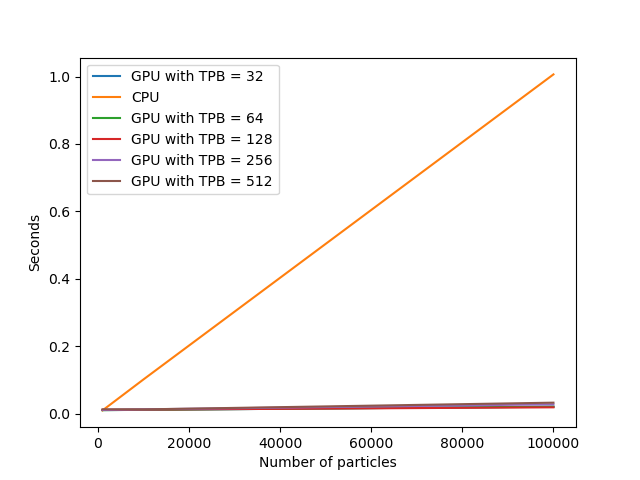
\includegraphics[scale=0.65]{fig.png}
  \end{center}
\item We can see from the graph the huge gap between the CPU and GPU results, and thus, a guess would be that even after doing a CPU dependent function, the GPU would still outperform the CPU, but not by much. One thing that is important to be remembered is the fact that copying data back and forth to and from the GPU is a costly action, since the transfer lanes for it are smaller and slower than with the resources of the GPU itself, when data is manipulated inside of the GPU. However, we can try to modify the code a bit and see if the graph proves us wrong or not:
  \begin{center}
    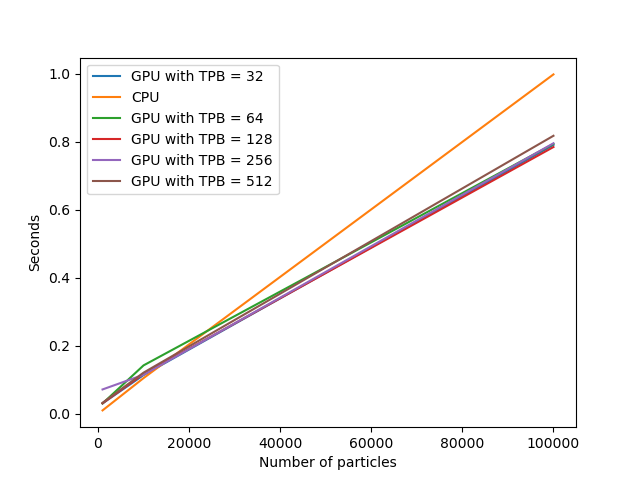
\includegraphics[scale=0.65]{fig2.png}
  \end{center}
  \noindent The results in the graph above show that with enough particles, the GPU still outpeforms the CPU, however, this time, the times are way closer than in the case where copying the data was only performed once.
\end{enumerate}

\clearpage 
\chapter{Bonus Exercise}
\section*{Calculating PI with CUDA}

The main difference between the GPU program compared to the CPU one is that all of the iterations that were run on the CPU are now individual threads on the GPU, and then each of them is now run a couple of times. One problem that we figured on the way is that the NUM\_ITER previously defined in the example code was higher than the total amount of allowed threads, thus we had to make that smaller, but not by much.

\begin{center}
  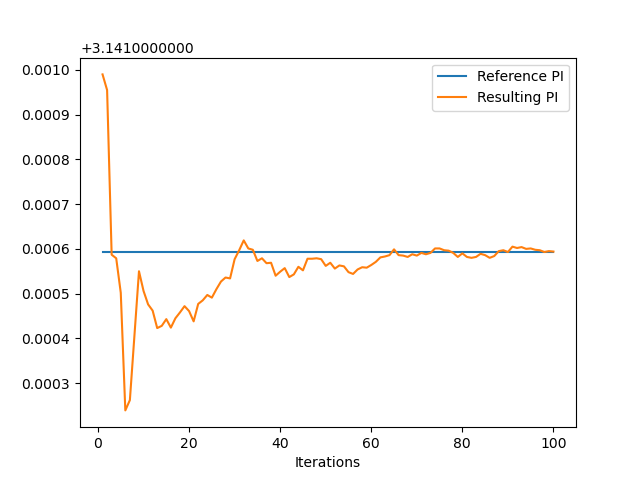
\includegraphics[scale=0.65]{plot3.png}
\end{center}


\begin{enumerate}
\item The number of threads we are using is 100000000 and we run the same approximation for a varying number of times on each thread, thus, the plot below:\\
  \begin{center}
    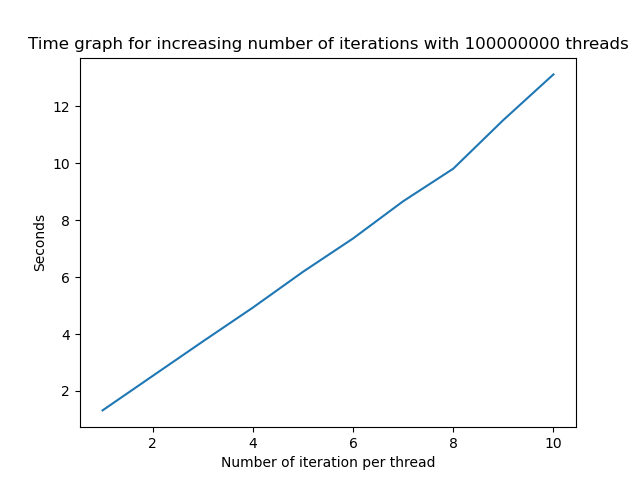
\includegraphics[scale=0.65]{plot1.png}
  \end{center}
  \begin{tabular}{ |p{6cm}||p{6cm}|  }
    \hline
    \multicolumn{2}{|c|}{GPU Pi computation times} \\
    \hline
    NUM\_ITERATIONS & Time (seconds)\\
    \hline
    1 & 1.354663\\
    2 & 2.511320\\
    3 & 3.709004\\
    4 & 4.982266\\
    5 & 6.143849\\
    6 & 7.357613\\
    7 & 8.570513\\
    8 & 9.745498\\
    9 & 10.907997\\
    10 & 12.236877\\
    \hline
  \end{tabular}

  \noindent We see that the times increase pretty much linearly with the increase of iterations.
\item Surprisingly enough, there is a clear winner when testing this, which is 16 threads per block. The results of the test are plotted in the image below: \\
  \begin{center}
    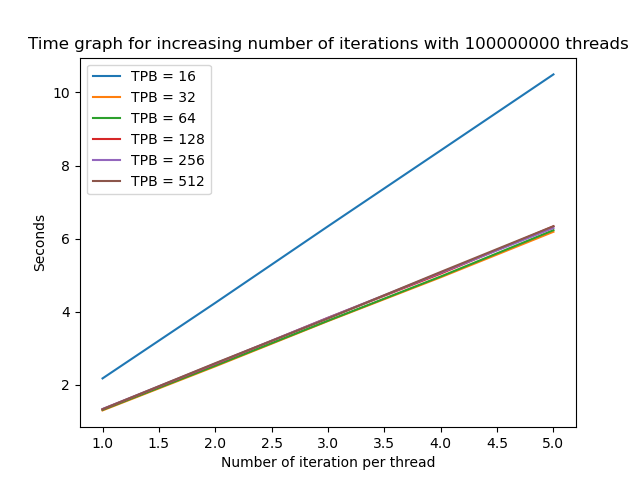
\includegraphics[scale=0.65]{plot2.png}
  \end{center}
\item The precision of the single precision values trastically decreased. The main reason for it is that the functions such as multiplication (when we power x and y by 2) or the square root will then act on rounded numbers (or less precise numbers). These are expected results, and the fact that the time performance was increased is also expected, since there are less calculations performed (because of less precision).\\\\
  \begin{center}
    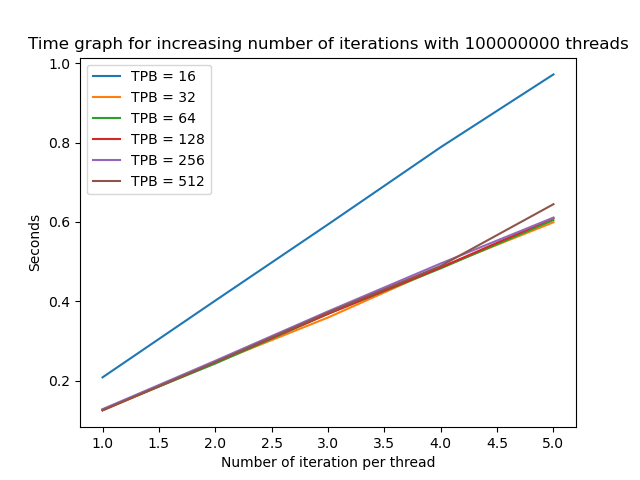
\includegraphics[scale=0.65]{plot4.png}
  \end{center}
  \noindent We can see in the plot above that, by running the exact same test as in the previous point, we get similar results. However, the total amount of time is somewhere in the order of 10 less!\\
  \begin{center}
    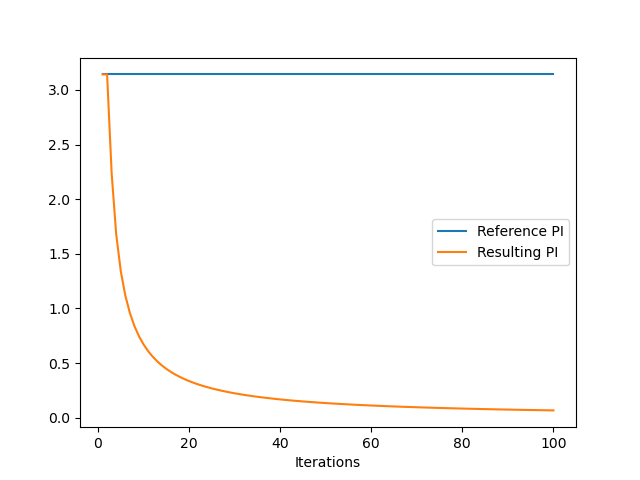
\includegraphics[scale=0.65]{plot5.png}
  \end{center}
  \noindent And finally, in the image above you can see that the accuracy decreased in an astonishing way.

\end{enumerate}

\clearpage 
\chapter{Appendix}

\ \\
\ \\
The source code is added here for all the exercises, however, here is also the clickable link to the github repository:\\\\
\url{https://github.com/capitanu/DD2360}
\\
\section*{Exercise 1 Code}


\begin{lstlisting}[style=CStyle]
#include <stdio.h>

#define TPB 256


__global__ void helloWorldKernel(){
	const int idx = blockIdx.x * blockDim.x + threadIdx.x;
	printf("Hello World! My threadId: %d\n", idx);
}

int main(){

	helloWorldKernel<<<1, TPB>>>();
	cudaDeviceSynchronize();
	return 0;
}

\end{lstlisting}

\section*{Exercise 2 Code}

\begin{lstlisting}[style=CStyle]
#include <stdio.h>
#include <stdlib.h>
#include <sys/time.h>

#define TPB 256

#define ARRAY_SIZE 1000000000

#define EPSILON 0.001

double cpuSecond() {
   struct timeval tp;
   gettimeofday(&tp,NULL);
   return ((double)tp.tv_sec + (double)tp.tv_usec*1.e-6);
}

__global__ void SAXPY_GPU(float *d_x, float *d_y, const float a){
	const int idx = threadIdx.x + blockDim.x * blockIdx.x;
	d_y[idx] = d_x[idx] * a + d_y[idx];
}

void SAXPY_CPU(float *x, float *y, const float a){
	for(int i = 0; i < ARRAY_SIZE; i++){
		y[i] = a*x[i] + y[i];
	}
}

int main(){

	float *x, *y, *y_gpu;
	x = (float *) malloc(sizeof(float) * ARRAY_SIZE);
	y = (float *) malloc(sizeof(float) * ARRAY_SIZE);
	y_gpu = (float *) malloc(sizeof(float) * ARRAY_SIZE);

	for(int i = 0; i < ARRAY_SIZE; i++){
		x[i] = rand() % 100;
		y[i] = rand() % 100;
	}
	float a = 3.45;
	
	float *d_x, *d_y;
	cudaMalloc(&d_x, sizeof(float) * ARRAY_SIZE);
	cudaMalloc(&d_y, sizeof(float) * ARRAY_SIZE);
	
	cudaMemcpy(d_x, x, sizeof(float) * ARRAY_SIZE, cudaMemcpyHostToDevice);
	cudaMemcpy(d_y, y, sizeof(float) * ARRAY_SIZE, cudaMemcpyHostToDevice);

	printf("Computing SAXPY on the CPU...");
	double start_cpu = cpuSecond();
	SAXPY_CPU(x,y,a);
	printf("Done! Took: %f seconds\n", cpuSecond() - start_cpu);

	printf("Computing SAXPY on the GPU...");
	double start_gpu = cpuSecond();
	SAXPY_GPU<<<(ARRAY_SIZE + TPB - 1)/TPB, TPB>>>(d_x, d_y, a);
	cudaDeviceSynchronize();
	printf("Done! Took: %f seconds\n", cpuSecond() - start_cpu);
	
	cudaMemcpy(y_gpu, d_y, sizeof(float) * ARRAY_SIZE, cudaMemcpyDeviceToHost);

	bool comp = true;
	for(int i = 0; i < ARRAY_SIZE; i++){
		if(abs(y[i] - y_gpu[i]) > EPSILON){
			comp = false;
			printf("%f\n", abs(y[i] - y_gpu[i]));
		}
	}

	cudaFree(d_x);
	cudaFree(d_y);
	
	free(y);
	free(x);
	free(y_gpu);
	
	printf("Comparing the output for each implementation...");
	if(comp)
		printf("Correct\n");
	else
		printf("Incorrect\n");
	
	

	return 0;
}
\end{lstlisting}

\section*{Exercise 3 Code}

\begin{lstlisting}[style=CStyle]
#include <stdio.h>
#include <stdlib.h>
#include <sys/time.h>
#include <cstdlib>

//#define NUM_PARTICLES 10000
//#define NUM_ITERATIONS 200
//#define TPB 64

struct Particle{
	float3 position;
	float3 velocity;
};

double cpuSecond() {
   struct timeval tp;
   gettimeofday(&tp,NULL);
   return ((double)tp.tv_sec + (double)tp.tv_usec*1.e-6);
}

__global__ void timestepKernel(Particle *d_particles, double3 randoms){
	const int idx = threadIdx.x + blockDim.x * blockIdx.x;

	d_particles[idx].velocity.x = randoms.x;
	d_particles[idx].velocity.y = randoms.y;
	d_particles[idx].velocity.z = randoms.z;

	d_particles[idx].position.x = d_particles[idx].position.x + d_particles[idx].velocity.x;
	d_particles[idx].position.y = d_particles[idx].position.y + d_particles[idx].velocity.y;
	d_particles[idx].position.z = d_particles[idx].position.z + d_particles[idx].velocity.z;
	
}

void timestepCPU(Particle *particles, double3 randoms, const int num_particles){
	for(int idx = 0; idx < num_particles; idx++){
				
		particles[idx].velocity.x = randoms.x;
		particles[idx].velocity.y = randoms.y;
		particles[idx].velocity.z = randoms.z;

		particles[idx].position.x = particles[idx].position.x + particles[idx].velocity.x;
		particles[idx].position.y = particles[idx].position.y + particles[idx].velocity.y;
		particles[idx].position.z = particles[idx].position.z + particles[idx].velocity.z;
	
	}
}

int main(int argc, char* argv[]){

	const int NUM_PARTICLES = atoi(argv[1]);
	const int NUM_ITERATIONS = atoi(argv[2]);
	const int TPB = atoi(argv[3]);

	const int BLOCK_SIZE = (NUM_PARTICLES + TPB - 1) / TPB;

	Particle *particles = (Particle *) calloc(NUM_PARTICLES, sizeof(Particle));
	Particle *d_particles;

	double3 rands;
	
	cudaMalloc(&d_particles, sizeof(Particle) * NUM_PARTICLES);


	double start_gpu = cpuSecond();
	cudaMemcpy(d_particles, particles, sizeof(Particle) * NUM_PARTICLES, cudaMemcpyHostToDevice);
	for(int i = 0; i < NUM_ITERATIONS; i++){

		rands.x = (double) rand() / (double) RAND_MAX;
		rands.y = (double) rand() / (double) RAND_MAX;
		rands.z = (double) rand() / (double) RAND_MAX;

		timestepKernel<<<BLOCK_SIZE, TPB>>>(d_particles, rands);
		cudaDeviceSynchronize();
	}
	cudaMemcpy(particles, d_particles, sizeof(Particle) * NUM_PARTICLES, cudaMemcpyDeviceToHost);
	printf("%f ", cpuSecond() - start_gpu);
	
	cudaFree(d_particles);
	
	double start_cpu = cpuSecond();
	for(int i = 0; i < NUM_ITERATIONS; i++){
		rands.x = (double) rand() / (double) RAND_MAX;
		rands.y = (double) rand() / (double) RAND_MAX;
		rands.z = (double) rand() / (double) RAND_MAX;
		timestepCPU(particles, rands, NUM_PARTICLES);
	}
	printf("%f\n", cpuSecond() - start_cpu);

	free(particles);

	
	return 0;
}
\end{lstlisting}

\section*{Bonus Exercise}
\begin{lstlisting}[style=CStyle]
#include <stdio.h>
#include <stdlib.h>
#include <sys/time.h>
#include <cstdlib>
#include <curand_kernel.h>
#include <curand.h>

//#define TPB         256
//#define NUM_ITER    10
#define SEED        921
#define NUM_THREADS 10000000

double cpuSecond() {
   struct timeval tp;
   gettimeofday(&tp,NULL);
   return ((double)tp.tv_sec + (double)tp.tv_usec*1.e-6);
}

__global__ void computeProbabilityKernel(curandState *states, int *d_count, int i){
	const int idx = threadIdx.x + blockDim.x * blockIdx.x;

	curand_init((SEED + i) * idx, idx, 0, &states[idx]);

	float x = curand_uniform(&states[idx]);
	float y = curand_uniform(&states[idx]);

	float z = sqrt((x*x) + (y*y));

	if(z <= 1.0){
		d_count[idx] = 1;
	}	
	
}

int main(int argc, char* argv[]){

	const int TPB = atoi(argv[2]);
	const int BLOCKS = (NUM_THREADS + TPB - 1)/TPB;
	const int NUM_ITER = atoi(argv[1]);

	curandState *d_random;
	cudaMalloc((void**)&d_random, TPB*BLOCKS*sizeof(curandState));

	int *count = (int*) calloc(BLOCKS*TPB, sizeof(int));
	int *d_count;
	cudaMalloc(&d_count, sizeof(int) * BLOCKS * TPB);


	float count_1s = 0;
	double start_gpu = cpuSecond();
	
	for(int i = 0; i < NUM_ITER; i++){

		for(int j = 0; j < TPB*BLOCKS; j++){
			count[j] = 0;
		}
		cudaMemcpy(d_count, count, sizeof(int) * BLOCKS * TPB, cudaMemcpyHostToDevice);

		computeProbabilityKernel<<<BLOCKS,TPB>>>(d_random, d_count, i);
		cudaDeviceSynchronize();
		
		cudaMemcpy(count, d_count, sizeof(int) * TPB * BLOCKS, cudaMemcpyDeviceToHost);

		for(int j = 0; j < BLOCKS*TPB; j++){
			if(count[j] == 1){
				count_1s += 1.0;
			}
		}

		float pi =  count_1s * 4.0 / ((float)(i+1) * (float) NUM_THREADS);
		printf("%f ", pi);
	}
	//printf("Time: %f seconds with %d threads and %d iterations per threads\n", cpuSecond() - start_gpu, NUM_THREADS, NUM_ITER);
	//printf("%f",cpuSecond()-start_gpu);
	//float pi =  count_1s * 4.0 / ((float) NUM_ITER * (float) NUM_THREADS);
	
    //printf("The result is %f\n", pi);
	
	return 0;
}  
\end{lstlisting}

\bibliographystyle{myIEEEtran}
\renewcommand{\bibname}{References}
\addcontentsline{toc}{chapter}{References}
\bibliography{references}

\end{document}
